%  BUILD:  pdflatex presentation_pf_sssa_ts_gfm_en.tex   (run twice for \inserttotalframenumber)
%
%  15-frame conference deck (16:9): in-house PF -> SSSA -> TS, proved against
%  PSAT on pure synchronous-machine cases FIRST, then the same stack carried to
%  four dual-mode converters and complete GFL/GFM switching.
%
%  HONESTY CONTRACT (docs/project/presentation/PRESENTATION_GUIDE.md):
%    * Every value is regenerated by the current in-house path and is covered by
%      a passing gate or a recorded cross-validation artifact. Each is carried
%      here with a % SOURCE: comment naming the file it was read from.
%    * PSAT 2.1.11 numbers come from the recorded three-way validation artifact
%      output/validation/artifacts/psat_pgaz_validation_2026-07-11_160014.md.
%    * No retired literature benchmark and no calibrated wrapper is presented as
%      validated physics; no literature range is used as an acceptance target.
%    * Powers of ten are typeset $a\times10^{n}$, never in e-notation.
%    * Switching scalars come from the generated macro files, so the prose here
%      cannot drift from the runs.
%    * Provenance note (DOC-2026-08-26-03): the trajectory presented is the
%      _zeta cache (inductive Thevenin DC link, 17 states). The only bit-identity
%      claimed anywhere in this deck is the measured agreement of the six arms on
%      the common window [0,20) s. No cross-model bit-identity is claimed.
\documentclass[aspectratio=169,10pt]{beamer}
\usepackage{amsmath,amsthm,amssymb}% amsthm BEFORE newtx: both define \openbox
\usepackage{newtxtext,newtxmath}
\usepackage{booktabs,array,tikz}
\usetikzlibrary{arrows.meta,positioning}
\usefonttheme{professionalfonts}

\definecolor{pnavy}{HTML}{0F2A4A}
\definecolor{pblue}{HTML}{1D5288}
\definecolor{pcyan}{HTML}{008080}
\definecolor{pgreen}{HTML}{1E7E34}
\definecolor{porange}{HTML}{D35400}
\definecolor{pred}{HTML}{A93226}
\definecolor{plight}{HTML}{F4F7FB}
\definecolor{pborder}{HTML}{CBD5E1}
\definecolor{pyellow}{HTML}{B7950B}

\setbeamercolor{normal text}{fg=pnavy,bg=white}
\setbeamercolor{frametitle}{fg=white,bg=pnavy}
\setbeamercolor{title}{fg=white}
\setbeamercolor{subtitle}{fg=white}
\setbeamercolor{structure}{fg=pblue}
\setbeamercolor{block title}{fg=pnavy,bg=pblue!12}
\setbeamercolor{block body}{fg=pnavy,bg=pblue!3}
\setbeamercolor{alertblock title}{fg=pred!90!black,bg=pred!14}
\setbeamercolor{alertblock body}{fg=pnavy,bg=pred!3}
\setbeamercolor{author in head/foot}{bg=pnavy,fg=white}
\setbeamercolor{date in head/foot}{bg=pnavy,fg=white}
\setbeamertemplate{blocks}[rounded][shadow=false]
\setbeamertemplate{navigation symbols}{}
\setbeamertemplate{itemize item}{\color{pblue}$\blacktriangleright$}
\setbeamertemplate{itemize subitem}{\color{pnavy!70}$\bullet$}
\setbeamersize{text margin left=5mm,text margin right=5mm}
% Figure lettering is Times New Roman 16 pt (pf_page_figure); body text is Times
% 16 pt, so the 1:1 include matches the surrounding text exactly.
\setbeamerfont{normal text}{size=\fontsize{13}{16}}
\setbeamerfont{frametitle}{size=\fontsize{18}{21},series=\bfseries}
\setbeamerfont{title}{size=\fontsize{24}{28},series=\bfseries}
\setbeamerfont{subtitle}{size=\fontsize{15}{18}}
\setbeamerfont{block title}{size=\fontsize{13}{16},series=\bfseries}
\setbeamerfont{block body}{size=\fontsize{12}{15}}
\setlength{\leftmargini}{1.2em}

\setbeamertemplate{footline}{%
  \leavevmode\hbox{\begin{beamercolorbox}[wd=.86\paperwidth,ht=2.4ex,dp=1.0ex,%
      leftskip=1em]{author in head/foot}%
    \scriptsize Automatic GFL/GFM Reference-Mode Switching
    \;\textbullet\; Department of Electrical Engineering, KMITL
    \end{beamercolorbox}\begin{beamercolorbox}[wd=.14\paperwidth,ht=2.4ex,dp=1.0ex,%
      center]{date in head/foot}%
    \scriptsize\insertframenumber/\inserttotalframenumber
    \end{beamercolorbox}}}

% Status badges: what supports each claim.
\newcommand{\pu}{\,\mathrm{p.u.}}
\newcommand{\gated}{\tikz[baseline=-0.6ex]\node[rounded corners=2pt,fill=pgreen!12,draw=pgreen,inner xsep=3pt,inner ysep=1pt]{\tiny GATED};}
\newcommand{\reported}{\tikz[baseline=-0.6ex]\node[rounded corners=2pt,fill=pblue!12,draw=pblue,inner xsep=3pt,inner ysep=1pt]{\tiny REPORTED};}
\newcommand{\openbadge}{\tikz[baseline=-0.6ex]\node[rounded corners=2pt,fill=porange!14,draw=porange,inner xsep=3pt,inner ysep=1pt]{\tiny OPEN};}

% Generated macros: the switching scalars cannot drift from the runs.
\IfFileExists{figures/switch_ieee14_decision/run_summary_v2.tex}%
  {% Generated by generate_ieee14_report_scalars. Do not edit.
%
% PROVENANCE. Accepted values of output/diagnostics/ieee14_gfm_lock_compare_dcreal/adaptive_250s.mat.
% Produced by run_ieee14_gfm_lock_comparison, whose option set is the
% flagship driver's plus agsi_reference=true (opt-in, post-processing only).
% This cache is NOT bit-identical to the earlier delivered artifact, and no
% such claim is made for it: the DC-link closure changed under
% NUM-2026-08-20-01, so the trajectory legitimately differs. Compare it to
% the earlier cache by outcome, never by bit-identity.
% No value here is rounded, scaled, smoothed or otherwise altered.
%
% Regenerate with:  pf_init_paths; generate_ieee14_report_scalars(result_file="output/diagnostics/ieee14_gfm_lock_compare_dcreal/adaptive_250s.mat")

\newcommand{\NewRunEnd}{250.000}
\newcommand{\NewRunVMin}{0.036855}
\newcommand{\NewRunVMax}{1.523183}
\newcommand{\NewRunFMin}{58.838795}
\newcommand{\NewRunFMax}{61.138560}
\newcommand{\NewRunSubdivision}{0}
\newcommand{\NewRunDomainRejects}{584}
\newcommand{\NewRunResidual}{$9.9596\times10^{-9}$}
\newcommand{\NewRunReclose}{159.240}
\newcommand{\NewRunRecloseStatus}{SUCCESS}
\newcommand{\NewRunSyncDV}{0.008785}
\newcommand{\NewRunSyncDF}{$6.4601\times10^{-13}$}
\newcommand{\NewRunSyncDTheta}{5.015017}
\newcommand{\NewRunFirstRelease}{25.310}
\newcommand{\NewRunReleaseOne}{25.310}
\newcommand{\NewRunReleaseTwo}{146.247}
\newcommand{\NewRunReleaseThree}{152.390}
\newcommand{\NewRunReleaseFour}{--}
\newcommand{\NewRunAugmentOne}{22.052}
\newcommand{\NewRunAugmentTwo}{51.333}
\newcommand{\NewRunAugmentThree}{53.372}
\newcommand{\NewRunAugmentFour}{148.267}
\newcommand{\NewRunNRelease}{3}
\newcommand{\NewRunNAugment}{4}
\newcommand{\NewRunGfmMax}{4}
\newcommand{\NewRunSamples}{4990}
\newcommand{\NewRunRejectedSteps}{135}
\newcommand{\NewRunTerminalF}{60.000000}
\newcommand{\NewRunTerminalVMin}{0.9667}
\newcommand{\NewRunTerminalVMax}{1.0575}
\newcommand{\NewRunStepper}{adaptive}
\newcommand{\NewRunReselection}{NO\_FEASIBLE\_SG\_ON\_ONE\_STEP}
}{}
\IfFileExists{figures/switch_ieee14_decision/comparison_macros.tex}%
  {% Generated by generate_ieee14_gfm_lock_comparison. Do not edit.
% Every number the comparison section prints comes from here, so the prose cannot drift
% from the runs. Arm keys: adaptive, pinned_gfm1, pinned_gfm2, pinned_gfm4, locked_gfl

\newcommand{\ArmAdaptiveLabel}{adaptive}
\newcommand{\ArmAdaptiveHorizon}{250.000}
\newcommand{\ArmAdaptiveConverged}{1}
\newcommand{\ArmAdaptiveReclose}{159.2397}
\newcommand{\ArmAdaptiveGfmMax}{4}
\newcommand{\ArmAdaptiveFailure}{--}
\newcommand{\ArmAdaptiveSamples}{4990}
\newcommand{\ArmAdaptiveRejected}{135}
\newcommand{\DfAdaptiveSGtrip}{0.7587}
\newcommand{\SetAdaptiveSGtrip}{0.0041}
\newcommand{\DfAdaptiveLoadstep}{1.0035}
\newcommand{\SetAdaptiveLoadstep}{0.3753}
\newcommand{\DfAdaptiveFault}{1.1386}
\newcommand{\SetAdaptiveFault}{0.3753}
\newcommand{\DfAdaptiveLinetrip}{0.3764}
\newcommand{\SetAdaptiveLinetrip}{0.3503}
\newcommand{\DfAdaptiveRestorereclose}{1.1612}
\newcommand{\SetAdaptiveRestorereclose}{0.0130}
\newcommand{\ArmPinnedgfmOneLabel}{pinned 1 GFM}
\newcommand{\ArmPinnedgfmOneHorizon}{250.000}
\newcommand{\ArmPinnedgfmOneConverged}{1}
\newcommand{\ArmPinnedgfmOneReclose}{151.4244}
\newcommand{\ArmPinnedgfmOneGfmMax}{1}
\newcommand{\ArmPinnedgfmOneFailure}{--}
\newcommand{\ArmPinnedgfmOneSamples}{3232}
\newcommand{\ArmPinnedgfmOneRejected}{542}
\newcommand{\DfPinnedgfmOneSGtrip}{0.5312}
\newcommand{\SetPinnedgfmOneSGtrip}{0.0113}
\newcommand{\DfPinnedgfmOneLoadstep}{1.4478}
\newcommand{\SetPinnedgfmOneLoadstep}{1.2214}
\newcommand{\DfPinnedgfmOneFault}{1.4979}
\newcommand{\SetPinnedgfmOneFault}{1.2296}
\newcommand{\DfPinnedgfmOneLinetrip}{1.2325}
\newcommand{\SetPinnedgfmOneLinetrip}{1.1426}
\newcommand{\DfPinnedgfmOneRestorereclose}{1.1736}
\newcommand{\SetPinnedgfmOneRestorereclose}{0.0210}
\newcommand{\ArmPinnedgfmTwoLabel}{pinned 2 GFM}
\newcommand{\ArmPinnedgfmTwoHorizon}{250.000}
\newcommand{\ArmPinnedgfmTwoConverged}{1}
\newcommand{\ArmPinnedgfmTwoReclose}{149.9191}
\newcommand{\ArmPinnedgfmTwoGfmMax}{2}
\newcommand{\ArmPinnedgfmTwoFailure}{--}
\newcommand{\ArmPinnedgfmTwoSamples}{3183}
\newcommand{\ArmPinnedgfmTwoRejected}{321}
\newcommand{\DfPinnedgfmTwoSGtrip}{0.3489}
\newcommand{\SetPinnedgfmTwoSGtrip}{0.0001}
\newcommand{\DfPinnedgfmTwoLoadstep}{0.7839}
\newcommand{\SetPinnedgfmTwoLoadstep}{0.7123}
\newcommand{\DfPinnedgfmTwoFault}{0.8255}
\newcommand{\SetPinnedgfmTwoFault}{0.7126}
\newcommand{\DfPinnedgfmTwoLinetrip}{0.7135}
\newcommand{\SetPinnedgfmTwoLinetrip}{0.6422}
\newcommand{\DfPinnedgfmTwoRestorereclose}{0.6634}
\newcommand{\SetPinnedgfmTwoRestorereclose}{0.0209}
\newcommand{\ArmPinnedgfmFourLabel}{pinned 4 GFM}
\newcommand{\ArmPinnedgfmFourHorizon}{25.491}
\newcommand{\ArmPinnedgfmFourConverged}{0}
\newcommand{\ArmPinnedgfmFourReclose}{--}
\newcommand{\ArmPinnedgfmFourGfmMax}{4}
\newcommand{\ArmPinnedgfmFourFailure}{\texttt{adaptiveDtMin}}
\newcommand{\ArmPinnedgfmFourSamples}{819}
\newcommand{\ArmPinnedgfmFourRejected}{449}
\newcommand{\DfPinnedgfmFourSGtrip}{0.9898}
\newcommand{\SetPinnedgfmFourSGtrip}{--}
\newcommand{\DfPinnedgfmFourLoadstep}{--}
\newcommand{\SetPinnedgfmFourLoadstep}{--}
\newcommand{\DfPinnedgfmFourFault}{--}
\newcommand{\SetPinnedgfmFourFault}{--}
\newcommand{\DfPinnedgfmFourLinetrip}{--}
\newcommand{\SetPinnedgfmFourLinetrip}{--}
\newcommand{\DfPinnedgfmFourRestorereclose}{--}
\newcommand{\SetPinnedgfmFourRestorereclose}{--}
\newcommand{\ArmLockedgflLabel}{locked GFL}
\newcommand{\ArmLockedgflHorizon}{20.000}
\newcommand{\ArmLockedgflConverged}{0}
\newcommand{\ArmLockedgflReclose}{--}
\newcommand{\ArmLockedgflGfmMax}{0}
\newcommand{\ArmLockedgflFailure}{\texttt{noVoltageFormingSource}}
\newcommand{\ArmLockedgflSamples}{43}
\newcommand{\ArmLockedgflRejected}{0}
\newcommand{\DfLockedgflSGtrip}{--}
\newcommand{\SetLockedgflSGtrip}{--}
\newcommand{\DfLockedgflLoadstep}{--}
\newcommand{\SetLockedgflLoadstep}{--}
\newcommand{\DfLockedgflFault}{--}
\newcommand{\SetLockedgflFault}{--}
\newcommand{\DfLockedgflLinetrip}{--}
\newcommand{\SetLockedgflLinetrip}{--}
\newcommand{\DfLockedgflRestorereclose}{--}
\newcommand{\SetLockedgflRestorereclose}{--}
\newcommand{\CommonWindowPinnedgfmOneBitIdentical}{1}
\newcommand{\CommonWindowPinnedgfmOneSamples}{42}
\newcommand{\CommonWindowPinnedgfmTwoBitIdentical}{1}
\newcommand{\CommonWindowPinnedgfmTwoSamples}{42}
\newcommand{\CommonWindowPinnedgfmFourBitIdentical}{1}
\newcommand{\CommonWindowPinnedgfmFourSamples}{42}
\newcommand{\CommonWindowLockedgflBitIdentical}{1}
\newcommand{\CommonWindowLockedgflSamples}{42}
\newcommand{\CommonWindowSplit}{20.000}
\newcommand{\CommonWindowAllBitIdentical}{1}
\newcommand{\CandTotal}{15}
\newcommand{\CandReady}{7}
\newcommand{\CandBestSet}{IBR3+IBR6}
\newcommand{\CandBestN}{2}
\newcommand{\CandBestOmega}{-0.56814}
\newcommand{\CandBestSingleOmega}{-0.32801}
\newcommand{\CandFullOmega}{-0.48291}
\newcommand{\CandReadyNOne}{4}
\newcommand{\CandTotalNOne}{4}
\newcommand{\CandReadyNTwo}{2}
\newcommand{\CandTotalNTwo}{6}
\newcommand{\CandReadyNThree}{0}
\newcommand{\CandTotalNThree}{4}
\newcommand{\CandReadyNFour}{1}
\newcommand{\CandTotalNFour}{1}
}{}

\title{An Automatic Following/Forming Framework for Inverter-Based Resources}
\subtitle{\texorpdfstring{PF--SSSA--TS analysis with automatic,\\
mathematically screened GFL/GFM reference-mode switching}%
{PF-SSSA-TS analysis with automatic, mathematically screened GFL/GFM reference-mode switching}}
\author{\texorpdfstring{Mr. Phichitchai Jueajan (66010569)\\Mr. Pakkapol Phdungdan (66010612)}%
{Mr. Phichitchai Jueajan (66010569); Mr. Pakkapol Phdungdan (66010612)}}
\institute{\texorpdfstring{Department of Electrical Engineering, Faculty of Engineering\\
King Mongkut's Institute of Technology Ladkrabang\\[2pt]
Advisor: Dr. Tossaporn Surinkaew}%
{Department of Electrical Engineering, Faculty of Engineering, KMITL; Advisor: Dr. Tossaporn Surinkaew}}
\date{11 September 2026}

\begin{document}

% ===========================================================================
\begin{frame}[plain]
  \begin{tikzpicture}[remember picture,overlay]
    \fill[pnavy] (current page.south west) rectangle (current page.north east);
    \fill[pcyan] (current page.south west) rectangle ([xshift=.16\paperwidth]current page.north west);
    \draw[white,opacity=.18,line width=1.2pt] ([xshift=.20\paperwidth,yshift=-.17\paperheight]current page.north west)
      -- ([xshift=.94\paperwidth,yshift=-.17\paperheight]current page.north west);
    \node[anchor=north east] at ([xshift=-0.28cm,yshift=-0.22cm]current page.north east)
      {
\includegraphics[width=0.62in]{figures/images.png}};
  \end{tikzpicture}
  \vspace{0.24cm}
  \hspace{1.15cm}\begin{minipage}{.81\textwidth}\raggedright
    {\usebeamerfont{title}\color{white}\inserttitle\par}
    \vspace{.14cm}
    {\usebeamerfont{subtitle}\color{white}\insertsubtitle\par}
    \vspace{.22cm}
    {\small\color{white!92}\insertauthor\par}
    \vspace{.08cm}
    {\footnotesize\color{white!84}\insertinstitute\par}
    \vspace{.08cm}
    {\footnotesize\color{white!84}\insertdate\par}
  \end{minipage}
\end{frame}

% ===========================================================================
\begin{frame}[shrink=4]{Problem, research question, and contributions}
\begin{columns}[T,onlytextwidth]
\column{.47\textwidth}
\begin{alertblock}{The operating problem}
\footnotesize
GFL converters need an external angle reference; GFM converters can create one,
but reserving every converter for GFM duty is costly and can introduce adverse
mode interaction. When the last synchronous reference trips, the operator must
decide more than simply ``GFL or GFM.''
\vspace{0.25em}
\begin{center}
\large\bfseries How many should form, which ones,\\and by what transition route?
\end{center}
\vspace{0.1em}
Two gaps matter: linear admissibility does not prove that the present state can
reach a configuration, and benefit is not monotone in the number of GFM units.
\end{alertblock}
\column{.49\textwidth}
\begin{block}{What this project contributes}
\begin{enumerate}\footnotesize
  \item One unified mathematical path from AC power flow through SSSA to
        switched time-domain simulation.
  \item A dual-mode coordinate superset with active-state projections and a
        current-continuity-gated GFL$\leftrightarrow$GFM assignment.
  \item Exhaustive screening of all $2^4-1=15$ non-empty GFM sets at their own
        equilibria, followed by transition certification.
  \item A five-policy falsification study: zero GFM is infeasible, four pinned
        GFM units hunt, and staged automatic switching completes $250$\,s.
\end{enumerate}
\vspace{0.1em}
{\scriptsize Motivation: Cui et al., \emph{IEEE TPS}, 2025; Ding et al.,
\emph{IEEE TSTE}, 2025.}
\end{block}
\end{columns}
\end{frame}

% ===========================================================================
\begin{frame}[shrink=6]{One mathematical stack: PF $\rightarrow$ SSSA $\rightarrow$ TS}
\begin{columns}[T,onlytextwidth]
\column{.48\textwidth}
\begin{block}{Network equilibrium and bus semantics}
\footnotesize
\vspace{-0.5em}\begin{align*}
F_{\mathrm{PF}}(z)&=0, & J_{\mathrm{PF}}\Delta z&=-F_{\mathrm{PF}},\\
g(x,V)&=Y_{\mathrm{net}}V-I_{\mathrm{bus}}(x,V)=0.
\end{align*}
\vspace{-0.2em}
REF fixes $|V|,\theta$; PV fixes $P,|V|$; PQ fixes $P,Q$.
IEEE-14 converges in $5$ Newton steps with
$\lVert F_{\mathrm{PF}}\rVert_\infty=6.34\times10^{-15}$\,pu.
\end{block}
\begin{block}{Exact DAE linearisation}
\footnotesize
\vspace{-0.5em}\begin{equation*}
\begin{bmatrix}\Delta\dot x\\0\end{bmatrix}=
\begin{bmatrix}f_x&f_y\\g_x&g_y\end{bmatrix}
\begin{bmatrix}\Delta x\\\Delta y\end{bmatrix},\qquad
A=f_x-f_y(g_y\backslash g_x).
\end{equation*}
One network-angle gauge coordinate is removed. Paired left/right eigenvectors
give participation; $\zeta=-\sigma/\sqrt{\sigma^2+\omega^2}$ is compared with
the declared $0.05$ floor.
\end{block}
\column{.48\textwidth}
\begin{block}{One coupled implicit time step}
\footnotesize
\vspace{-0.5em}\begin{align*}
R_x&=x_{n+1}-x_n-\frac{h}{2}
  [f(x_n,y_n)+f(x_{n+1},y_{n+1})]=0,\\
R_y&=g(x_{n+1},y_{n+1})=0.
\end{align*}
Damped Newton solves both residuals together. Adaptive step doubling estimates
local error; accepted steps land exactly on scheduled events. Domain-invalid
trials are rejected and unresolved transitions fail closed.
\end{block}
\begin{block}{A switch is an assignment, not a time step}
\footnotesize
Inactive controller coordinates are re-initialised at the current terminal
operating point. Commit requires
$\lVert I^+-I^-\rVert_\infty\le10^{-10}$\,pu and a right-limit KCL solve.
\end{block}
\end{columns}
\end{frame}

% ===========================================================================
\begin{frame}[shrink=5]{Defensible decision parameters}
\begin{columns}[T,onlytextwidth]
\column{.49\textwidth}
\begin{block}{Normalised severity and hysteresis}
\footnotesize
\vspace{-0.45em}\begin{align*}
J_V&=\frac{\bigl||V_i|-V_i^\star\bigr|}{0.10\,\mathrm{pu}}, &
J_f&=\frac{|f_{\mathrm{COI}}-60|}{0.50\,\mathrm{Hz}},\\
S&=\mathrm{sat}_{[0,1]}\!\left(\tfrac12J_V+\tfrac12J_f\right).
\end{align*}
\vspace{0em}
Equal weights combine local voltage and system frequency after normalisation.
The hysteresis and dwell conditions are
\begin{align*}
S\ge0.65&\ \text{for}\ 0.10\,\mathrm{s} &&(\mathrm{GFL}\to\mathrm{GFM}),\\
S<0.35&\ \text{for}\ 1.00\,\mathrm{s} &&(\mathrm{GFM}\to\mathrm{GFL}).
\end{align*}
The gap prevents chatter; the unequal dwell makes support fast and release slow.
\end{block}
\column{.47\textwidth}
\begin{block}{Prediction frozen before measurement}
\footnotesize
The non-ideal DC source is specified as a second-order, maximally-flat response:
\begin{equation*}
\zeta^\star=\frac{1}{\sqrt2},\qquad \tau_s=5.00\,\mathrm{ms}.
\end{equation*}
This predicts, before the assembled spectrum is evaluated,
\begin{equation*}
f\approx15.5\,\mathrm{Hz},\qquad \zeta=0.7071.
\end{equation*}
The measured four-converter result is
\begin{equation*}
f=15.18\text{--}15.66\,\mathrm{Hz},\qquad
\zeta=0.7072\text{--}0.7079.
\end{equation*}
The agreement is therefore a prediction check, not parameter fitting.
\end{block}
\begin{alertblock}{Interpretation rule}
\footnotesize Parameter consequences are checked after selection; no parameter,
event or acceptance threshold is changed in response to the observed curves.
\end{alertblock}
\end{columns}
{\scriptsize Mathematical bases: IEEE Std 1110; Kundur (1994); Kodsi--Ca\~nizares
(2003); MATPOWER IEEE-14 data; stated project derivations.}
\end{frame}

% ===========================================================================
\begin{frame}{Independent validation I: power flow and small signal}
\begin{block}{Identical mapped inputs: proposed framework vs PSAT 2.1.11 \gated}
\vspace{-0.6em}\begin{center}\footnotesize
\begin{tabular}{llrr}\toprule
quantity & pair & IEEE 14 & RTS-24 \\ \midrule
network contract $\max|\Delta Y|$ & Ours$-$PSAT & $3.97\times10^{-15}$ & $2.84\times10^{-14}$ \\
power flow $\max|\Delta V|$ [pu] & PSAT$-$Ours & $6.661338\times10^{-16}$ & $4.441\times10^{-16}$ \\
power flow $\max|\Delta\theta|$ [deg] & PSAT$-$Ours & $3.552714\times10^{-14}$ & $6.750\times10^{-14}$ \\
\bottomrule\end{tabular}
\end{center}\vspace{-0.5em}
% SOURCE: output/validation/artifacts/psat_pgaz_validation_2026-07-11_160014.md:39,45,54,60
\footnotesize Tolerances declared \emph{before} the comparison:
$\Delta V<10^{-6}$\,pu, $\Delta\theta<10^{-4}$\,deg. The required gate passes
with ten orders of magnitude to spare --- the two solvers agree at machine
precision, not merely within a tolerance.
\end{block}
\begin{block}{Small signal, five-machine classical IEEE 14 \gated}
\footnotesize
Four oscillatory modes give
$|\Delta\lambda|=1.000\times10^{-6}$\,s$^{-1}$ on \emph{every} mode. This
uniform offset is the documented regularisation of the reference analysis;
the physical frequencies match to the printed precision:
$1.83350$, $1.58440$, $1.53137$, $1.35374$\,Hz on both sides.
% SOURCE: figures/padiyar_two_area/table_ieee14_sssa_ours_psat.tex (all four rows);
%         shift documented at report_padiyar_two_area.tex:955-957
\end{block}
\end{frame}

% ===========================================================================
\begin{frame}{Validation II: transient trajectories}
\begin{columns}[T,onlytextwidth]
\column{.52\textwidth}
\begin{block}{Proposed framework vs PSAT 2.1.11 (IEEE 14-bus) \gated}
\vspace{-0.6em}\begin{center}\footnotesize
\begin{tabular}{lrr}\toprule
Metric & Max Difference & Tolerance Gate \\ \midrule
$\Delta\delta_{\text{COI}}$ [deg] & $9.571\times10^{-3}$ & $< 0.05$ \\
$\Delta\omega$ [pu] & $3.816\times10^{-6}$ & $< 1.0\times10^{-4}$ \\
$\Delta P_e$ [MW] & $4.217\times10^{-2}$ & $< 0.10$ \\
$\Delta|V|$ (fault bus) [pu] & $3.179\times10^{-5}$ & $< 1.0\times10^{-3}$ \\
\bottomrule\end{tabular}
\end{center}\vspace{-0.5em}
% SOURCE: case14_ts_compare_three_way.md:26 (IEEE-14 row)
\footnotesize
Pre-declared tolerances on dynamic state trajectories are satisfied across the
full 15\,s simulation horizon with substantial margin.
\end{block}
\column{.46\textwidth}
\begin{block}{Trajectory Agreement Insights}
\footnotesize
\begin{itemize}
  \item \textbf{Close trajectory agreement}: Generator rotor angles $\delta_{\text{COI}}$,
        speeds $\omega$, active power outputs $P_e$, and bus voltages $|V|$
        closely trace PSAT reference trajectories throughout fault and post-fault periods.
  \item \textbf{Acceptance evidence}: The complete comparison horizon contains
        zero unconverged steps and every measured difference remains inside its gate.
  \item \textbf{Validated baseline}: Establishes an independent reference on
        classical machines before incorporating advanced dual-mode IBR converters.
\end{itemize}
\end{block}
\end{columns}
\vspace{0.3em}
\centering\small Every pre-declared PSAT trajectory gate is satisfied before the analysis is extended to dual-mode IBR converters.
\end{frame}

% ===========================================================================
\begin{frame}{Same network, four converters, one switching contract}
\begin{columns}[T,onlytextwidth]
\column{.50\textwidth}
\footnotesize
The PSAT validation ran classical machines at buses $1,2,3,6,8$.
% SOURCE: psat_pgaz_validation_2026-07-11_160014.md:38
This study keeps the machine at bus~1 and replaces buses $2,3,6,8$ by four
dual-mode converters on the same network and operating base.
\vspace{0.3em}
\begin{block}{One coordinate layout, two regimes --- exclusive}
\footnotesize
\vspace{-0.4em}\begin{center}\footnotesize
\begin{tabular}{lrl}\toprule
grid-following & 10 active & 7 controller states frozen \\
grid-forming & 11 active & 6 controller states frozen \\
tripped & 0 active & everything held \\
\bottomrule\end{tabular}
\end{center}\vspace{-0.4em}
% SOURCE: +ibr/eecon49_dual_mode_model.m:95-96 (index 17 appended to both sets when n_src==1)
17 coordinates per converter; composite $6+4\times17=74$ coordinates. The
17-vector is a \emph{superset}, not a simultaneously active state: only the
selected controller branch evolves in each regime.
\end{block}
\column{.46\textwidth}
\begin{block}{The transfer itself}
\footnotesize
A mode change is an \emph{assignment}, not a trapezoidal step, and it commits
only if terminal current is continuous to $10^{-10}$. The parameterisation may
jump; the current the network sees cannot.
% SOURCE: report_ieee14_switch_en_rev2.tex:1502 (eq:assign), :1127-1140 (transfer, continuity)
\end{block}
\begin{block}{The severity index that triggers it}
\footnotesize
\vspace{-0.7em}\begin{equation*}
S=\mathrm{sat}_{[0,1]}\!\left(\tfrac12 J_V+\tfrac12 J_f\right)
\end{equation*}
\vspace{-1.0em}
\begin{equation*}
J_V=\frac{\bigl||V_i|-V_i^\star\bigr|}{0.10\pu},\qquad
J_f=\frac{|f_{COI}-60|}{0.50\,\mathrm{Hz}}
\end{equation*}
$V_i^\star$ is the healthy power-flow voltage; the equal weighting is a project
choice frozen before any result was read. Commit at $S\ge0.65$ held $0.10$\,s;
release at $S<0.35$ held $1.00$\,s --- quick to add support, deliberately slow
to release it. Four further sub-indices are computed but kept diagnostic: they
enter no gate and form no aggregate by design.
% SOURCE: :467-485 (index, bases, weighting tag), :491-499 (thresholds), :256-261 (diagnostic four)
\end{block}
\end{columns}
\end{frame}

% ===========================================================================
% RESERVED: the owner supplies a hand-drawn network diagram for this frame.
\begin{frame}{Study network}
\centering
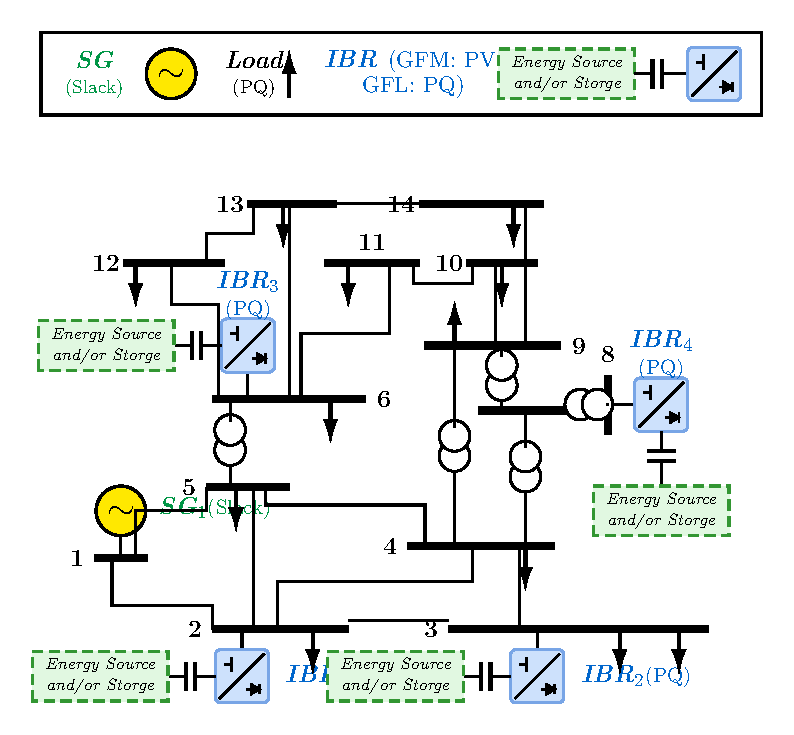
\includegraphics[height=2.62in]{figures/ieee14_dual_mode_ibr_diagram.pdf}
\vspace{-0.2em}

\scriptsize The SG holds the healthy-system angle reference. After its trip, an
authenticated GFM converter must own the island reference; all devices remain
coupled through $g(x,V)=Y_{net}V-I_{bus}(x,V)=0$.
\end{frame}

% ===========================================================================
\begin{frame}[shrink=6]{The spectrum, at the two operating points that matter}
\begin{columns}[T,onlytextwidth]
\column{.49\textwidth}
\begin{block}{Machine online, all converters following}
\footnotesize
$44$ physical coordinates of $45$ (one angle removed by the network-angle
quotient). The electromechanical mode is the one the case contract speaks about:
\vspace{-0.3em}\begin{center}
\begin{tabular}{lr}\toprule
$\lambda$ & $-1.146045\pm7.254946\mathrm{j}$ \\
$f$ & $1.154661$\,Hz \\
$\zeta$ & $0.156033$ \\
dominant state & machine speed \\
\bottomrule\end{tabular}
\end{center}\vspace{-0.3em}
against the declared floor $\zeta_{\min}=0.05$ --- a factor of three of margin.
Slowest root $-0.174920$ (machine field flux).
% SOURCE: figures/switch_ieee14/sssa_sg_on_modes_all_gfl.tex:2 (44 of 45), :40 (row 30), :44 (SG1:Eqp)
\end{block}
\column{.49\textwidth}
\begin{block}{Machine tripped, one converter forming}
\footnotesize
$40$ physical of $41$; $30$ printed rows, conjugate pairs once; \emph{entirely}
in the left half plane --- the island the converters hold is small-signal stable.
\vspace{-0.3em}\begin{center}
\begin{tabular}{lrr}\toprule
 & $\lambda$ & dominant \\ \midrule
fastest & $-2075.371442$ & inner current \\
DC family & $-98.41\pm98.38\mathrm{j}$ & DC link \\
 & \dots\,3 more pairs & DC link \\
PLL pair & $-0.588912\pm2.171749\mathrm{j}$ & PLL angle \\
slowest & $-0.328014\pm0.448860\mathrm{j}$ & voltage loop \\
\bottomrule\end{tabular}
\end{center}
% SOURCE: figures/switch_ieee14/sssa_modes_n1.tex:2 (40 of 41), :11, :20, :38, :40
The slowest root \emph{is} the decay-rate margin the selector ranks on.
\end{block}
\end{columns}
\vspace{0.2em}
\begin{alertblock}{Two limits stated, not buried \openbadge}
\footnotesize
$9$ of the $30$ rows have their two leading participations within $0.02$, so the
named state there is \emph{not} a sole attribution --- every table carries that
mark per row. And this is one linearisation point: it is not, and must not be
read as, a stability certificate for the switched trajectory.
% SOURCE: sssa_modes_n1.tex:43 (dagger footnote); report_ieee14_switch_en_rev2.tex:1574-1576
\end{alertblock}
\end{frame}

% ===========================================================================
\begin{frame}[shrink=4]{Predicted first, then measured: the DC link}
\begin{columns}[T,onlytextwidth]
\column{.48\textwidth}
\begin{block}{What was predicted, before the run}
\footnotesize
The converter's DC side was an ideal source. Replacing it by a real source
behind a resistance and an inductance adds one state per converter, and its time
constant is not free: requiring the flattest possible response fixes the damping
at $\zeta^\star=1/\sqrt2$ and therefore the time constant at $5.00$\,ms. From
that alone the pole pair was predicted, on paper, at
\vspace{-0.3em}\begin{center}
$-97.7\pm97.7$\,s$^{-1}$, \quad $f\approx15.5$\,Hz, \quad $\zeta=0.7071$.
\end{center}\vspace{-0.3em}
Two feasibility bounds were declared at the same time, and the realised margin
against the binding one is $2.07$--$2.15$. The source voltage is not chosen
either --- the dispatch forces it, giving $1.0269$--$1.0448\pu$ across the four
converters.
% SOURCE: report_ieee14_switch_en_rev2.tex:918-975 (tau_s, zeta, bounds, Edc range), :898
\end{block}
\column{.48\textwidth}
\begin{block}{What the assembled system then returned \gated}
\footnotesize
\vspace{-0.3em}\begin{center}
\begin{tabular}{lrr}\toprule
 & predicted & measured \\ \midrule
$f$ [Hz] & $\approx15.5$ & $15.18$--$15.66$ \\
$\zeta$ & $0.7071$ & $0.7072$--$0.7079$ \\
\bottomrule\end{tabular}
\end{center}\vspace{-0.2em}
Four converters, four pairs, every one of them where the derivation said it
would be. Participation splits exactly $0.500/0.500$ between the two DC
coordinates and is $0.000$ everywhere else, so each pair \emph{is} one
converter's DC circuit and nothing else.
% SOURCE: :1588-1590 (four pairs), :1595-1604 (participation)
\end{block}
\begin{alertblock}{And the coupling was measured, not assumed \openbadge}
\footnotesize
The AC equations read the DC states with sensitivity \emph{exactly zero}; the DC
equations do read the AC. The coupling is one-way --- which also means a sagging
DC link never limits an AC command in this model, so nothing here covers
DC-limited ride-through.
% SOURCE: :1609-1615 (eq:oneway), :1621-1630 (property of this model)
\end{alertblock}
\end{columns}
\end{frame}

% ===========================================================================
\begin{frame}[shrink=4]{How many converters, and which --- computed}
\begin{columns}[T,onlytextwidth]
\column{.52\textwidth}
\begin{block}{Candidate Set Admissibility}
\vspace{-0.3em}\begin{center}\footnotesize
\begin{tabular}{clrl}\toprule
size & grid-forming set & margin [s$^{-1}$] & outcome \\ \midrule
1 & bus 8 & $-0.155437$ & admissible \\
1 & bus 6 & $-0.252025$ & admissible \\
1 & bus 3 & $-0.316711$ & admissible \\
1 & bus 2 & $-0.328014$ & admissible \\
2 & buses 2 + 6 & $-0.561723$ & admissible \\
2 & \textbf{buses 3 + 6} & $\mathbf{-0.568138}$ & \textbf{best} \\
2 & four other pairs & -- & limit hit \\
3 & all four triples & -- & no equilibrium \\
4 & all converters & $-0.482909$ & admissible \\
\bottomrule\end{tabular}
\end{center}\vspace{-0.3em}
\end{block}
% SOURCE: figures/switch_ieee14/sssa_candidate_summary.tex:10-24 (all 15 rows, Omega and reason)
\column{.46\textwidth}
\begin{block}{What the enumeration proves}
\footnotesize
\CandTotal{} candidate sets evaluated, \CandReady{} admissible ---
\CandReadyNOne{} of \CandTotalNOne{} at size 1,
\CandReadyNTwo{} of \CandTotalNTwo{} at size 2,
\CandReadyNThree{} of \CandTotalNThree{} at size 3,
\CandReadyNFour{} of \CandTotalNFour{} at size 4.
% SOURCE: comparison_macros.tex:125-139
\begin{itemize}\footnotesize
  \item \textbf{Non-monotonic}: 1-GFM sets pass, 3-GFM fail, optimum sits at 2-GFM ($-0.5681$\,s$^{-1}$).
  \item \textbf{Optimal pairing}: Buses 3 + 6 outperform single or 4-converter configurations.
  \item \textbf{Analytical proof}: Sizing cannot follow heuristic rules of thumb; must be rigorously computed.
\end{itemize}
\end{block}
\begin{alertblock}{Necessary, not sufficient \openbadge}
\footnotesize
The 4-converter set passes the linear SSSA screen yet \emph{fails} dynamically: pinned from the trip it terminates at $t=\ArmPinnedgfmFourHorizon$\,s due to unmitigated hunting.
% SOURCE: report_ieee14_switch_en_rev2.tex:1656-1658, :1786-1787; comparison_macros.tex:60
\end{alertblock}
\end{columns}
\end{frame}

% ===========================================================================
\begin{frame}{The disturbance chronology: six periods}
\begin{center}
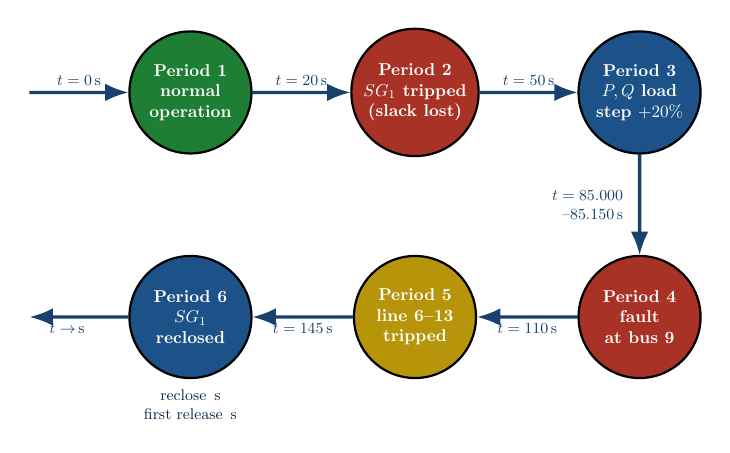
\begin{tikzpicture}[
  scale=0.62,transform shape,
  per/.style={circle,draw,thick,minimum size=2.5cm,inner sep=2pt,
    align=center,text=white,font=\bfseries},
  tlbl/.style={font=\small},
  tlab/.style={midway,above,font=\small},
  tlabb/.style={midway,below,font=\small},
  arr/.style={-{Latex[length=3mm]},very thick,color=pblue!80!black}]
\node[per,fill=pgreen] (p1) at (0,0)     {Period 1\\ normal\\ operation};
\node[per,fill=pred]   (p2) at (4.6,0)   {Period 2\\ $SG_1$ tripped\\ (slack lost)};
\node[per,fill=pblue]  (p3) at (9.2,0)   {Period 3\\ $P,Q$ load\\ step $+20\%$};
\node[per,fill=pred]   (p4) at (9.2,-4.6){Period 4\\ fault\\ at bus 9};
\node[per,fill=pyellow](p5) at (4.6,-4.6){Period 5\\ line 6--13\\ tripped};
\node[per,fill=pblue]  (p6) at (0,-4.6)  {Period 6\\ $SG_1$\\ reclosed};
\draw[arr] (-3.3,0) -- node[tlab]{$t=0$\,s} (p1);
\draw[arr] (p1) -- node[tlab]{$t=20$\,s} (p2);
\draw[arr] (p2) -- node[tlab]{$t=50$\,s} (p3);
\draw[arr] (p3) -- node[font=\small,left=2mm,pos=0.5,align=right]{$t=85.000$\\--$85.150$\,s} (p4);
\draw[arr] (p4) -- node[tlabb]{$t=110$\,s} (p5);
\draw[arr] (p5) -- node[tlabb]{$t=145$\,s} (p6);
\draw[arr] (p6) -- node[tlabb,pos=0.62]{$t\to\NewRunEnd$\,s} ++(-3.3,0);
\node[tlbl,below=3pt of p6,align=center,text=pnavy]
  {reclose $\NewRunReclose$\,s\\ first release $\NewRunFirstRelease$\,s};
\end{tikzpicture}
\end{center}
\vspace{-0.2em}
\footnotesize Green: undisturbed. Red: a contingency that removes a source or
faults a bus. Yellow: a topology change. Blue: a restorative action. The six
scheduled instants are case-defined; the reclose and first release instants are
\emph{read from the accepted event log} of the run --- they are results, not
inputs.
\end{frame}

% ===========================================================================
\begin{frame}{The supervisor's decision, over the whole run}
\begin{center}
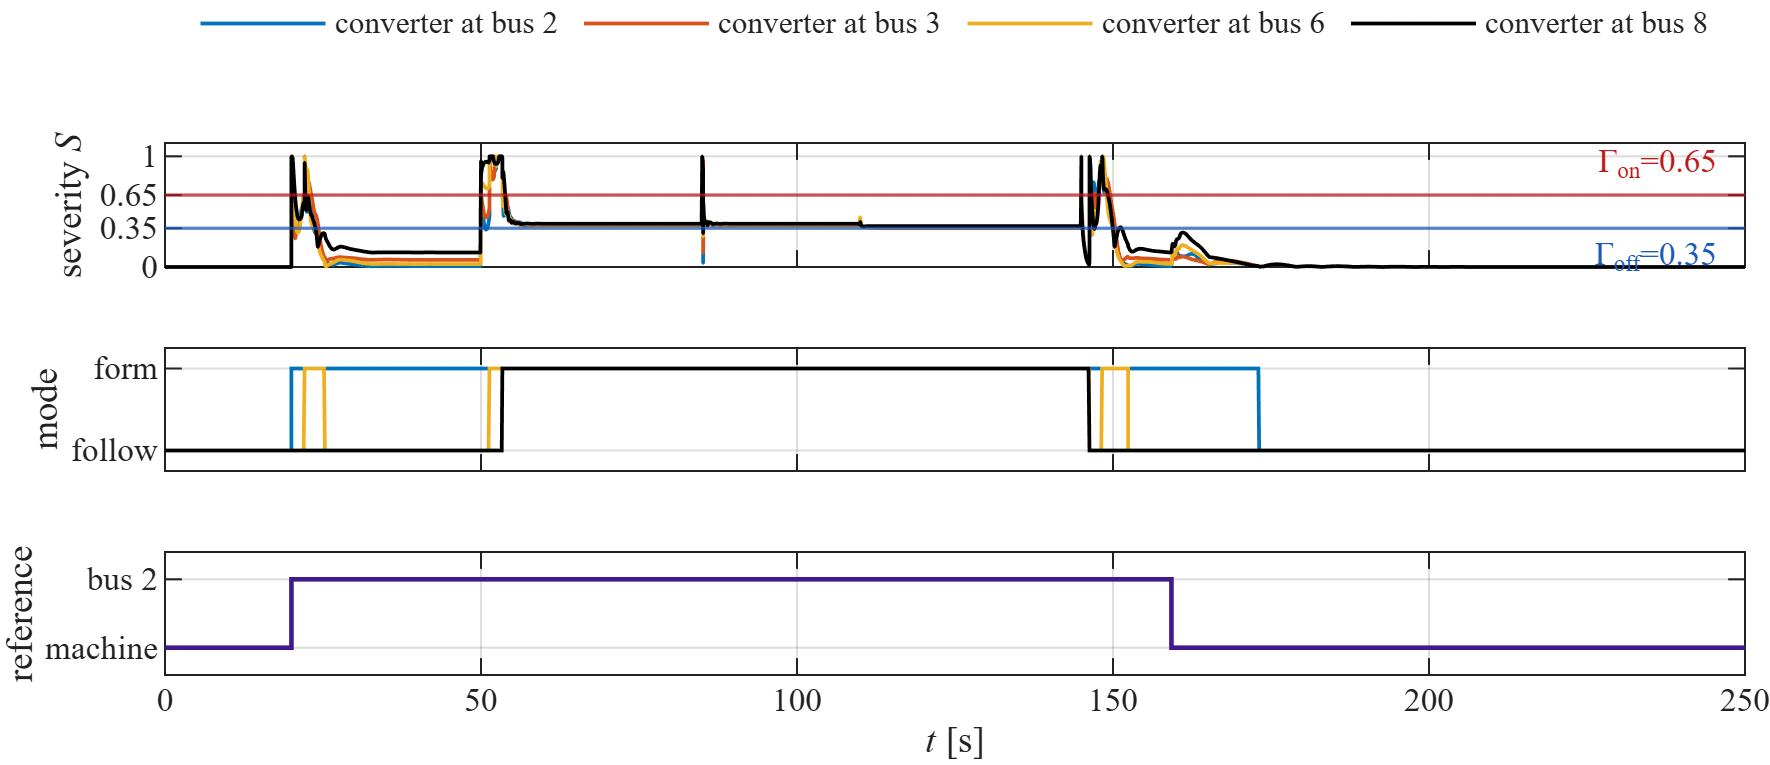
\includegraphics[width=5.90in]{figures/presentation_pf_sssa_ts_gfm/slide_supervisor.png}
\end{center}
\vspace{-0.4em}
\footnotesize
The severity index crosses the commit threshold \emph{only} at the disturbances,
and the asymmetric dwell prevents chatter. Peak commitment is
$\NewRunGfmMax{}$ converters; the run ends with \emph{none} grid-forming and the
machine holding the reference again.
% SOURCE: slide_supervisor.png from generate_presentation_switch_figure (zeta cache);
%         run_summary_v2.tex:22,42
\end{frame}

% ===========================================================================
\begin{frame}{Electrical response on the same time axis}
\begin{center}
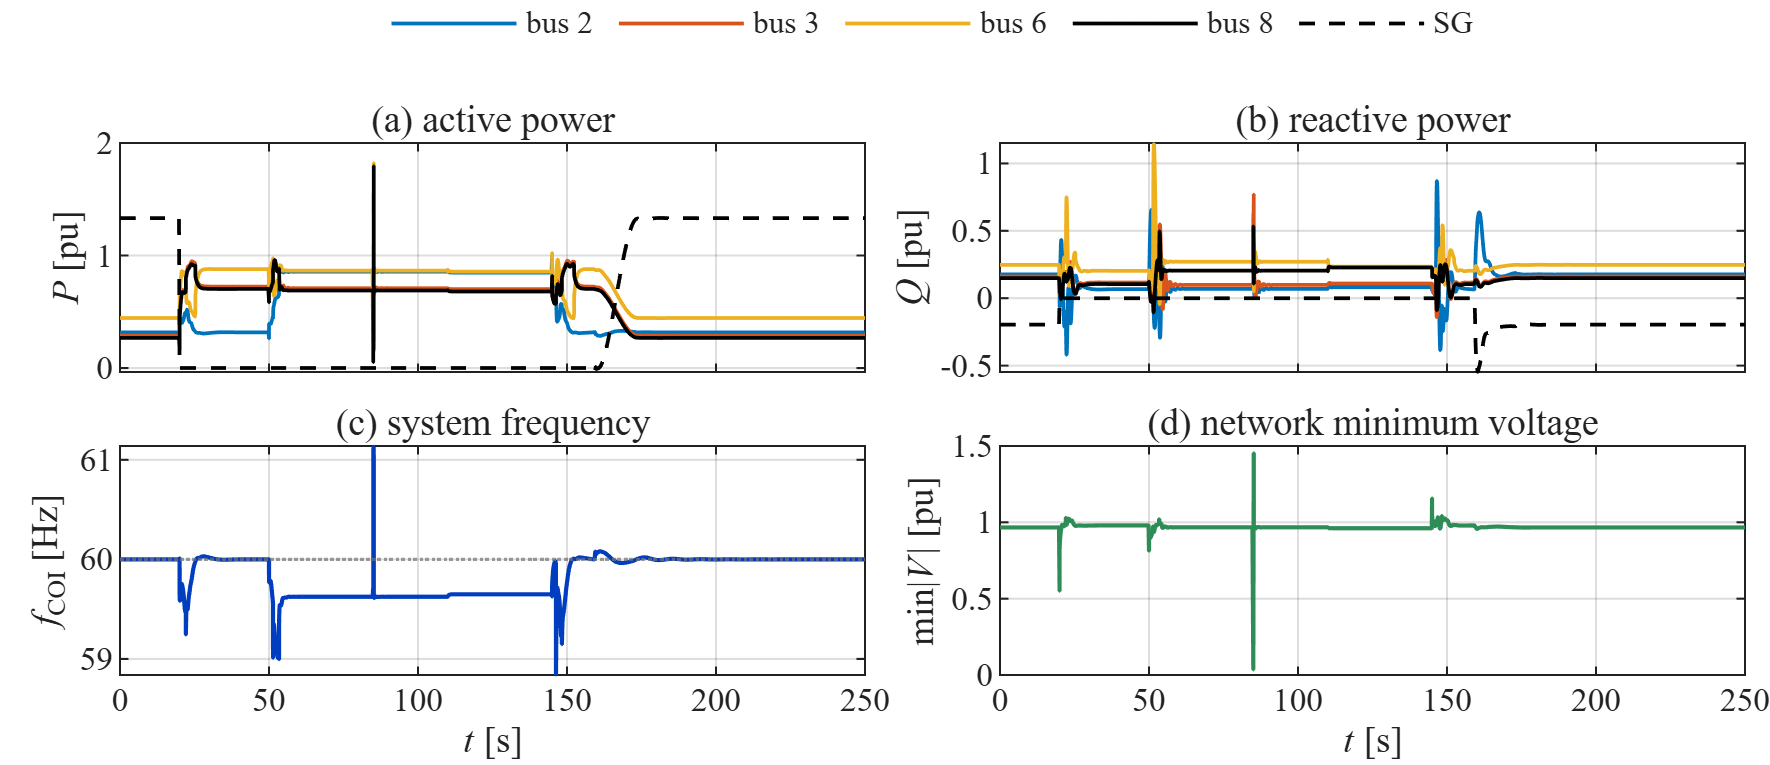
\includegraphics[width=5.70in]{figures/presentation_pf_sssa_ts_gfm/slide_electrical.png}
\end{center}
\vspace{-0.7em}
\scriptsize
The machine (dashed) drops to zero at the trip and returns at the reclose; the
converters take up the difference. Frequency shows both under- and overshoot at
the disturbances, then recovers to $\NewRunTerminalF$\,Hz. Voltage collapses only during the bolted
fault and returns to $\NewRunTerminalVMin$--$\NewRunTerminalVMax\pu$.
% SOURCE: slide_electrical.png from generate_presentation_switch_figure; run_summary_v2.tex:45-47
\end{frame}

% ===========================================================================
\begin{frame}[shrink=10]{Switching is necessary, not merely better}
\begin{center}
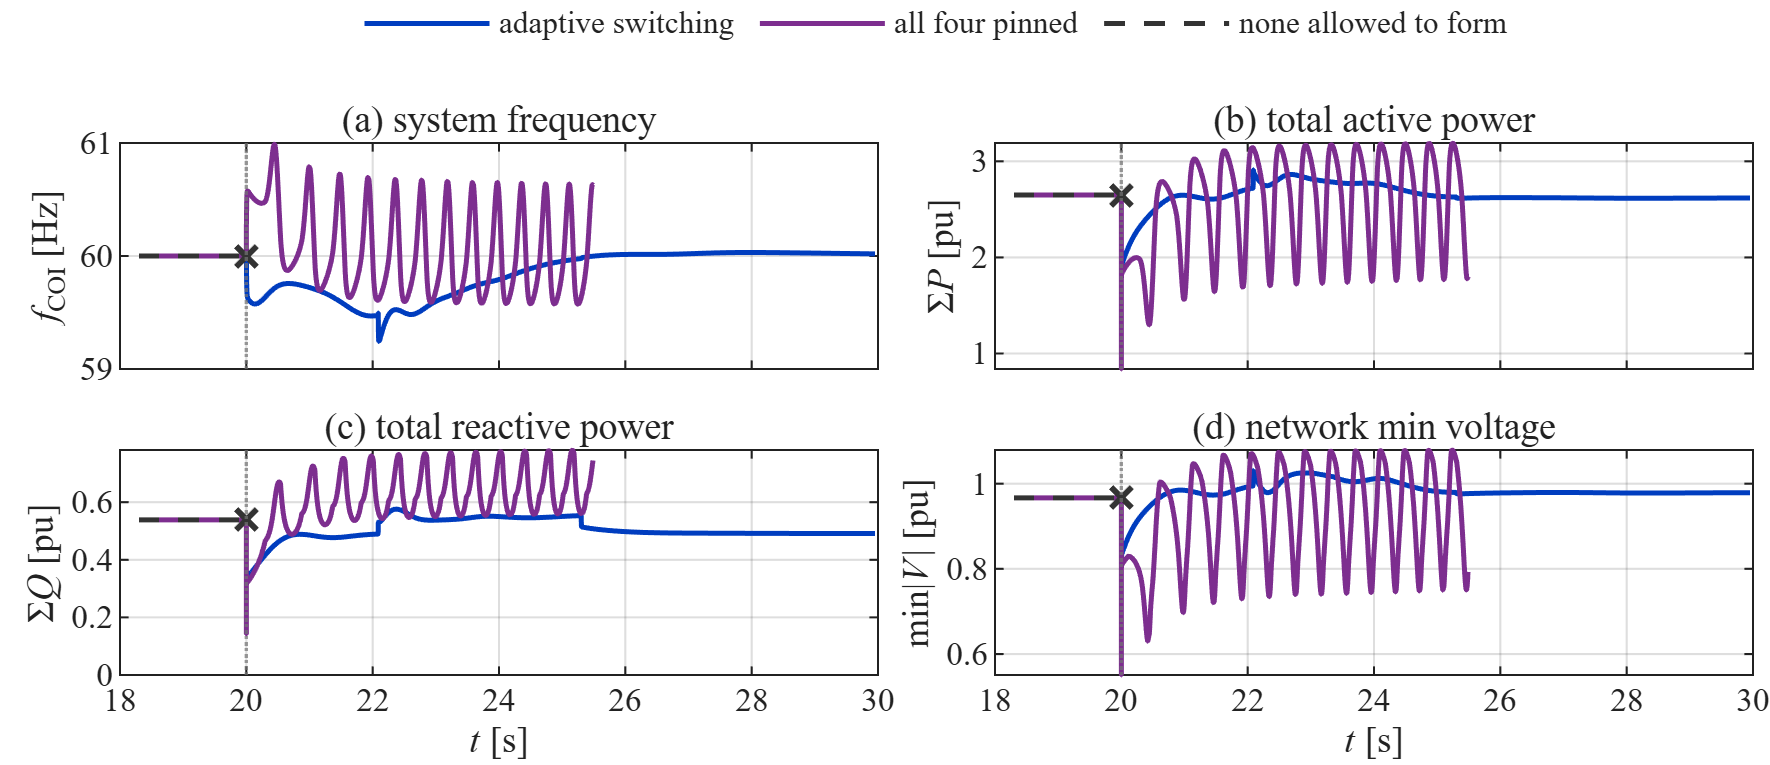
\includegraphics[width=5.32in]{figures/presentation_pf_sssa_ts_gfm/slide_necessity.png}
\end{center}
\vspace{-0.7em}
\begin{columns}[T,onlytextwidth]
\column{.49\textwidth}
\footnotesize
\textbf{None allowed to form} --- with zero voltage-forming capability, the post-trip solve is \emph{refused} at $t=20\text{ s}$ (\ArmLockedgflSamples{} samples).
\textbf{All four pinned} --- rigid GFM mode interaction causes rapid power and frequency hunting, terminating at $t=\ArmPinnedgfmFourHorizon$\,s.
\textbf{Adaptive switching} --- rides through all six scheduled disturbance events.
\column{.47\textwidth}
\footnotesize
\textbf{Multi-signal dynamic evidence}:
\begin{itemize}\footnotesize
  \item Frequency $f_{\text{COI}}$ settles cleanly at nominal 60\,Hz without hunting.
  \item Total power $(\Sigma P,\Sigma Q)$ shares the islanded load while
        $\min|V|$ recovers after each cleared contingency.
  \item Settled deviation improved by $3.28\times$ vs static GFM during fault.
\end{itemize}
% SOURCE: comparison_summary.tex:49-53,60; comparison_macros.tex:13-22,49-58,83
\end{columns}
\end{frame}

% ===========================================================================
\begin{frame}[shrink=5]{Established here --- and openly not claimed}
\begin{columns}[T,onlytextwidth]
\column{.48\textwidth}
\begin{block}{Established \gated}
\begin{itemize}\small
  \item power flow and time-domain results agree with an independent
        third-party tool on two networks, under tolerances declared in advance
        --- power flow at machine precision. The same gate \emph{refuses} a
        second third-party tool, and that refusal is printed
  \item the composite Jacobian's block structure follows from a proposition
        with an \emph{iff} converse, not from an assumed sparsity pattern
  \item on this resource mix at least one grid-forming converter is
        \emph{necessary} for a post-trip trajectory to exist at all
  \item the admissible grid-forming set is non-monotone in its size, with an
        interior optimum --- so it must be computed, not assumed
  \item the 250\,s chronology closes: the machine recloses on merit, every
        converter is handed back, and the terminal frequency lands within
        $10^{-6}$\,Hz of nominal
\end{itemize}
\end{block}
\column{.48\textwidth}
\begin{alertblock}{Not claimed \openbadge}
\begin{itemize}\small
  \item \textbf{no operational readiness} --- convergence is not grid-code
        compliance, and the extrema are model excursions, not ratings
  \item \textbf{no selector-against-selector} claim: this is switching against
        \emph{not} switching, on this resource mix
  \item \textbf{no multi-machine} result --- that path fails closed at four
        points and no numbers are assumed in their place
  \item four of the six severity sub-indices are kept diagnostic: they enter
        no gate and form no aggregate by design
  \item the DC mode sits at the resolution limit of a phasor method; a firmer
        link belongs to an electromagnetic-transient study
  \item unresolved model limitations are disclosed explicitly and none is used
        to support an operational-readiness claim
\end{itemize}
\end{alertblock}
\end{columns}
% SOURCE: report_ieee14_switch_en_rev2.tex:242-281 (the not-claimed block);
%         docs/project/defects/INDEX.md (IBR-2026-07-20-01, AGSI-2026-08-14-01, TEST-2026-08-13-04)
\end{frame}

\end{document}
